\documentclass{article}
\usepackage[utf8]{inputenc}
\usepackage[margin=1in]{geometry}
\usepackage{sectsty}
\usepackage{indentfirst}
\usepackage[super]{nth}
\usepackage{graphicx}
\usepackage{subfig}
\usepackage{caption}
\usepackage{subcaption}

\title{An Analysis of the Applications of Computer Vision on Identifying Lost Dogs}
\author{Aidan Vickars, Anant Sunilam Awasthy, Karthik Srinatha, and Rishabh Kausha}
\date{\today}

\begin{document}

\maketitle

\newpage
\section{Motivation and Background}
As the most common house pet in the world by a large margin, lost dogs are a frequent problem around the world; dogs are family and as a result losing a dog even for a minute can be one of the scariest times of a persons life.  With this is mind, it stands to reason their is no shortage of interest in new techniques for finding a lost dog.  Of course, there are a variety classical of methods for finding a lost dog.  These include posting lost posters on telephone poles near ones location, posting adds on Craiglist and social media sites as well as leveraging web applications such as the "BC SPCA Pet Search" run by the British Columbia Society for the Prevention of Cruelty to Animals (BCSPCA).  However, all of these methods require creating some form of a eye catching poster that have been used in so many different forms that they have lost their intended affect.  As a result, a new method is needed.  Thus, in this paper we will present a data pipeline implemented as an Android Application that leverages three separate convolutional neural networks to match dogs marked as lost with dogs marked as found and vice versa by computing the similarity between lost and found dogs and subsequently returning the results.

To measure the success of our pipeline we devised a test by randomly designating 1000 dogs from the test portion of our custom data-set as "lost", and randomly designating 100 of these "lost" dogs as "found", and subsequently applied our data pipeline on these dogs.  We found that using our current hyper-parameters, our model matched the "lost" dogs with the "found" 100\% of the time (ADD REAL STAT HERE).  Our data collecting, processing procedures, models are all presented, and the source code has been made publicly available.

\section{Related Work}
While dog-identification is a sub-class of the heavily researched facial recognition area, dog-identification remains extremely undeveloped.  However, there are two related works that we discuss here.  The first is "A Deep Learning Approach for Dog Face Verification and Recognition" (CITATION)  by  Guillaume Mougeit, Dewei Li and Shuai Jia.  In "A Deep Learning Approach for Dog Face Verification and Recognition", Mougeit, Li and Jia present "VGG-like and "ResNet-like" (page 422) models to encode the image of a dog to $\mathbb{R}^n$ and compute the Euclidean distance between the encoding of two images to produce a probability.  This probability is used to perform face verication to determine if two dogs are the same.  To quantify the accuracy of their models they generated 2500 positive pairs and 2500 negative pairs images of various dog faces.  In this scenario positive indicates the images represent the same dog and negative indicates the images represent different dogs.  Their models made the correct decision 92\% and 91\% of the time for each model respectively.

The second work is "Dog Identification using Soft Biometrics and Neural Networks" (CITATION) by Kenneth Lai, Xinyuan Tu and Svetlana Yanushkevich.  In "Dog Identification using Soft Biometrics and Neural Networks", Lai, Tu and Yanushkevich present an approach to increase the accuracy in dog-identification that is inspiration behind the work presented here, and all credit is given to them with respect to similarities between works.  Lai, Tu and Yanushkevich developed an dog detection model, a breed classification model, and dog-identification model that work together in the order specified.   The dog detection model determines the bounding box of the face of a dog and can be used to crop the image accordingly.  The breed classification model like other models of this type, simply determines the likely breed of the dog.  Finally, the dog-identification model functions in the same way as that of  Mougeit, Li and Jia (CITATION) and encodes the image of a dog to $\mathbb{R}^n$ and the Euclidean distance between the encodings of two dogs is used to quantiy the similarity between the dogs.  By first cropping the image, and determining the breed of the dog, the number of comparisons that are made using the dog-identification model is significantly reduced and improves the face verification accuracy.  However, we do not list accuracy of the models as the dog-identification model is trained on the "Flickr-dog" dataset that contains only 374 images made up of just two breeds.  As a result, our results are incomparable.

\section{Problem Statement}
It should be noted that in both related works discussed above, the dog-identification or face-verification models leverage only the face of a dog.  That is the entire body of the dog is cropped and only the face is given to the model.  This presents a problem or deficiency in two ways.  The first is that by training the model on a data set that appears to be highly curated and contains only front facing dog faces, the crucial assumption is made that all applicable images of dogs all contain the dog's face in a relatively front facing fashion.  This is obviously not the case.  As any dog owner knows, convincing your dog two look at the camera is a non-trivial task and that the majority of their photos are of the dog in an appealing position with their face obscured.  An example of this is shown in Figure \ref{fig:x dog no face} below.  The second, is the by cropping the image to only the dogs face we theorize that valuable 


\begin{figure}[h]
\centering
	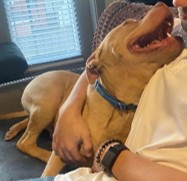
\includegraphics{final-report-images/nofacedog.jpg}
\caption{An Example of a Dog with their Face Obscured}
\label{fig:x dog no face}
\end{figure}
The second, is the by cropping the image to only the dogs face we theorize that valuable information is lost.  In the case of face verification in humans,only examining the face is reasonable and desirable because humans change clothes.  However, dogs do not.  We certainly note that there are cases where dogs do where clothes but these cases are infrequent.  Thus, we theorize that by leveraging a dogs entire dog we may see an improvement in the accuracy of the dog-identification model relative to work done by  Lai, Tu and Yanushkevich because the model could leverage additional characteristics such as the size of the dog.  This is illustrated in Figures \ref{fig:similar faces} and \ref{fig:different bodies} where in Figure 2 we see two dogs with similar faces.  One could forgive a model for classifying these dogs as the same.  But as shown in Figure 3 we can clearly see that are not.  By leveraging the entire body of dog, this miss-classification should be eliminated.

\begin{figure}[h]
\centering
	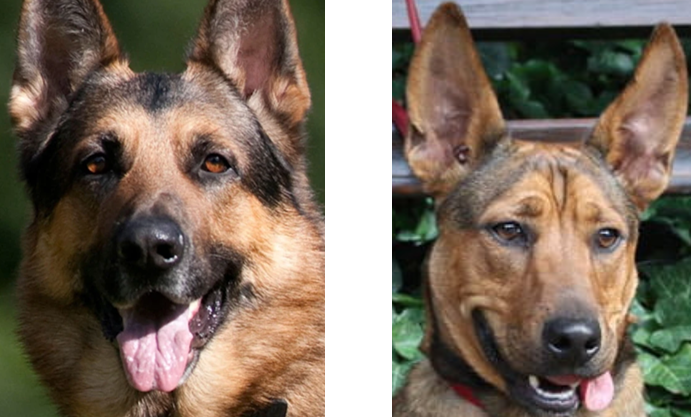
\includegraphics{final-report-images/similar_faces.png}
\caption{Sample Images of Two Dogs with Similar Faces}
\label{fig:x similar faces}
\end{figure}

\newpage

\begin{figure}[h]
\centering
	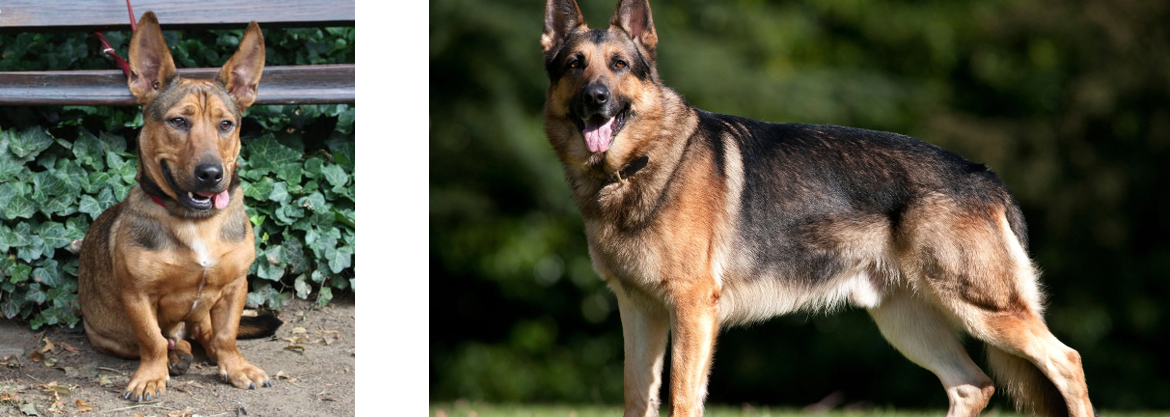
\includegraphics{final-report-images/different_bodies.png}
\caption{Sample Images of Two Dogs with Different Bodies}
\label{fig:x different bodies}
\end{figure}

Thus, we can now present the key problems this project aims to answer:

\begin{enumerate}
  \item By leveraging the entire body of a dog, can we construct an dog-identification model that can accurately determine if two dogs are the same or note?  Furthermore, by incorporating the entire body of a dog, can we achieve a better accuracy than that achieved by Mougeit, Li and Jia?
  \item By removing the restriction of curated front facing dogs, can we construct a pipeline that can accurately match lost dogs with found dogs and vice versa? 
\end{enumerate}

\section{Data Science Pipeline}

To answer the questions stated above, we use the work done by Mougeit, Li and Jia and constructed a similar VGG model to compare dogs and we also incorporate the work done by Lai, Tu and Yanushkevich and construct a dog-detection model and a breed classification to improve accuracy.  In future references we refer to the these models as the Dog Comparator, the Dog Classifier and the Dog Extractor respectively.   We can now break down the data science pipeline into individual components with respect to the data used to develop each model respectively.

For the Dog Extractor model, we utilize the "Open Images" data-set that contains thousands of images of dogs with corresponding bounding boxes.  While this data is already relatively clean, we discard all grey-scale images, and convert all images not already in RGB format to RGB.  The decision was made to discard grey-scale images because our expectation is that in the production environment of our Data Product that is discussed below, the vast majority of images will be colour images.  After cleaning this left 19 995 training images, 1568 validation images , and 4791 test images.

For the Dog Classifier Model ---------------------

Now, to train the Dog Comparator model we required multiple pictures of many individual dogs where each picture contained the entire body of the dog.  We found that there was no data-set that met these requirements.  We note that the "Stanford Dog Dataset" exists that contains multiple imags of 1425 individual dogs.  However, each image contained only the face of a dog and the images appeared to be highly curated.  Which as discussed above, we feel is undesirable.  To solve this we scraped the trove of images on Petfinder.com that at the time of writing lists over 100 000 for adoption across the world where almost every dog has multiple images.  However, scraping the images presented a challenge because the links to every dog are dynamically generated.  To be succinct, scraping the HTML of the web page containing the grid of available dogs using Python's request package was not sufficient because during download the URLs pointing to each available dog would not be included due to their dynamic creation.  To solve this, we split the scraping into two parts.  We first created a Selenium application in Python that scrapes the URLs pointing to each individual dog.  Then, using these URLs we scraped and downloaded the images for every dog and also recorded additional information such as name, breed, age, size etc.  This resulted in images for 9729 dogs with 0 - 6 images for every dog.  Once the data was downloaded, we applied the following cleaning process on the images of every dog:

\begin{enumerate}
  
  \item If the dog has 1 or a less images, we discarded the dog and its images
  
  \item Confirm every image was in RGB format or convert it to RGB format.  Otherwise the image was discarded.
  
  \item Passed every image into the Dog Extractor Model:
    \begin{itemize}
      \item Verify if the image contained a dog
      \item Verify if the image contained only one dog
      \item Record the bounding box coordinates of the dog
    \end{itemize}
    If either of the conditions in the first two bullets were not met, the image was discarded.
    
  \item If after the previous step, the Dog had 1 or less images we discarded the dog and its images.
  
\end{enumerate}

\noindent After cleaning we were left with 8349 dogs with 2 - 6 images for every dog.  The data set was then divided into a Train, Validation and Test split of 70\%, 10\%, and 20\% respectively.  This gave a total of 6679 training dogs, 501 validation dogs and 1169 testing dogs respectively.  We do note that we did not account for the actual number of dog images contained in each split.  This is because during the training and testing process we only considered the images on a dog by dog bases.  This will become more clear in the presentation of the Dog Comparator model below.

\section{Methodology}
Within this section we discuss the approaches used in each model.  For all three models, we present the architecture used in and their respective results.  We also perform a deep analysis into their strength and weaknesses.  With respect to the first model, the Dog Extractor model we discuss the two approaches taken and their failure and success respectively.

\subsection{Dog Extractor}

\subsubsection{Initial Approach}

\subsubsection{Final Approach}

\subsection{Dog Classifier}


\section{Data Product}

To answer the questions stated above, we use the work done by Mougeit, Li and Jia and use similar VGG model to compare dogs and we also incorporate the work done by Lai, Tu and Yanushkevich and use additional models to improve accuracy.  We further extend this by using the entire body of a dog instead of the face to improve accuracy.  To utulize this work in a production environment, we have created an android application (app) to act as user interface to allow for easy image upload, and have packaged the models into a Flask API (API) to perform matchings between lost and found dogs. We also use an AWS S3 bucket and a Relational Database System (RDS) to store images and image metadata respectively.  This system is visualized below in Figure \ref{fig:x app system}.

\begin{figure}[h]
\centering
	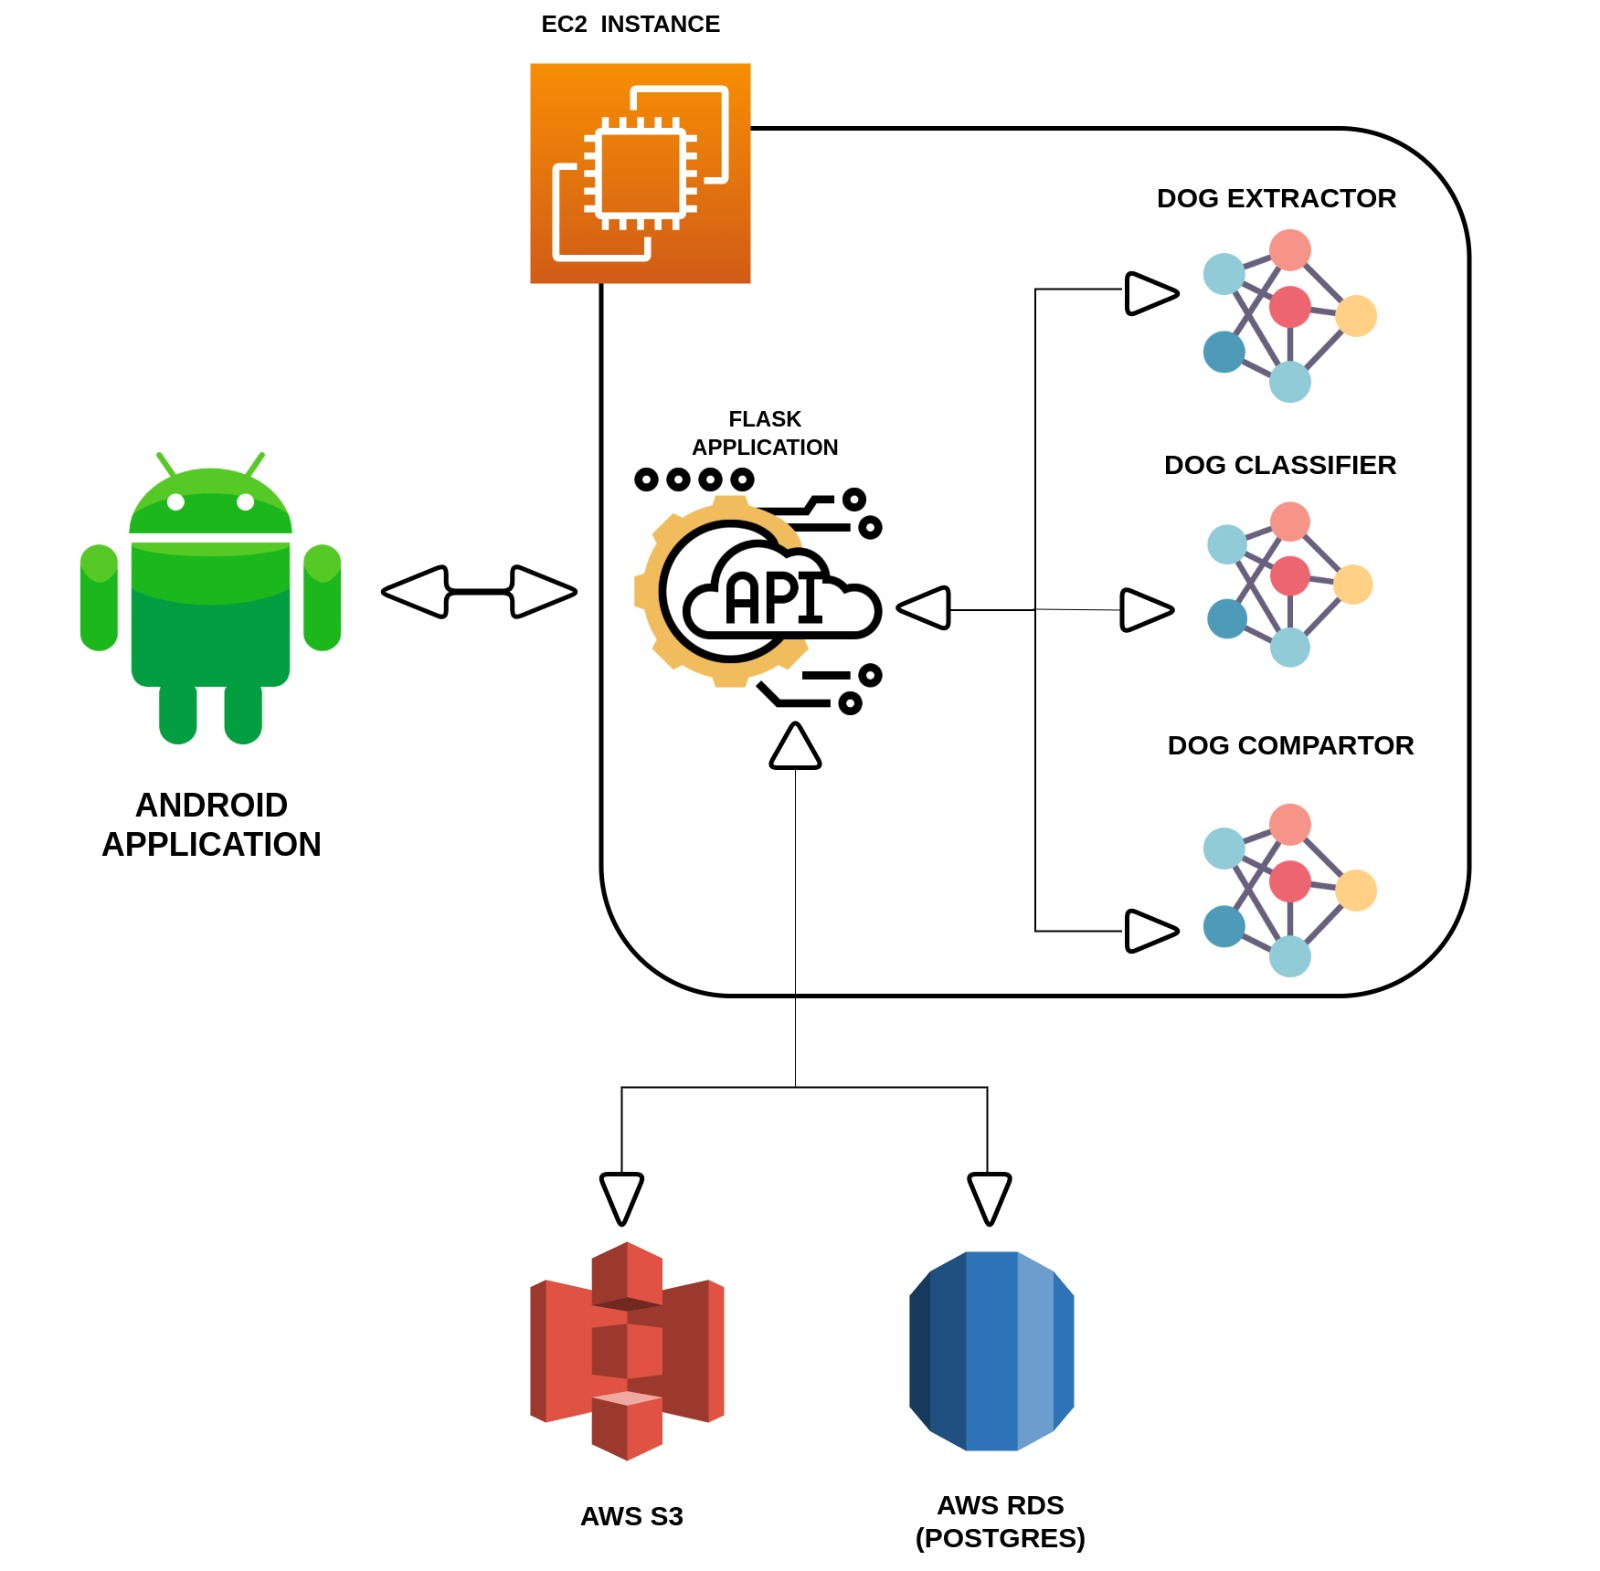
\includegraphics[scale=0.1]{final-report-images/system.jpeg}
\caption{Dog Finder System}
\label{fig:x app system}
\end{figure}

At a lower level we will now explain how the entire system works as visualized in Figure: \ref{fig:x app pipeline}.  Initially, if a user has lost a dog, they will submit a photo and as well as their contact information and location via the app.  The app will then submit this information to the API.  Once a submission has been made to the API, the dog finder pipeline is triggered.  The following steps outline this pipeline:

\newpage

\begin{figure}[h]
\centering
	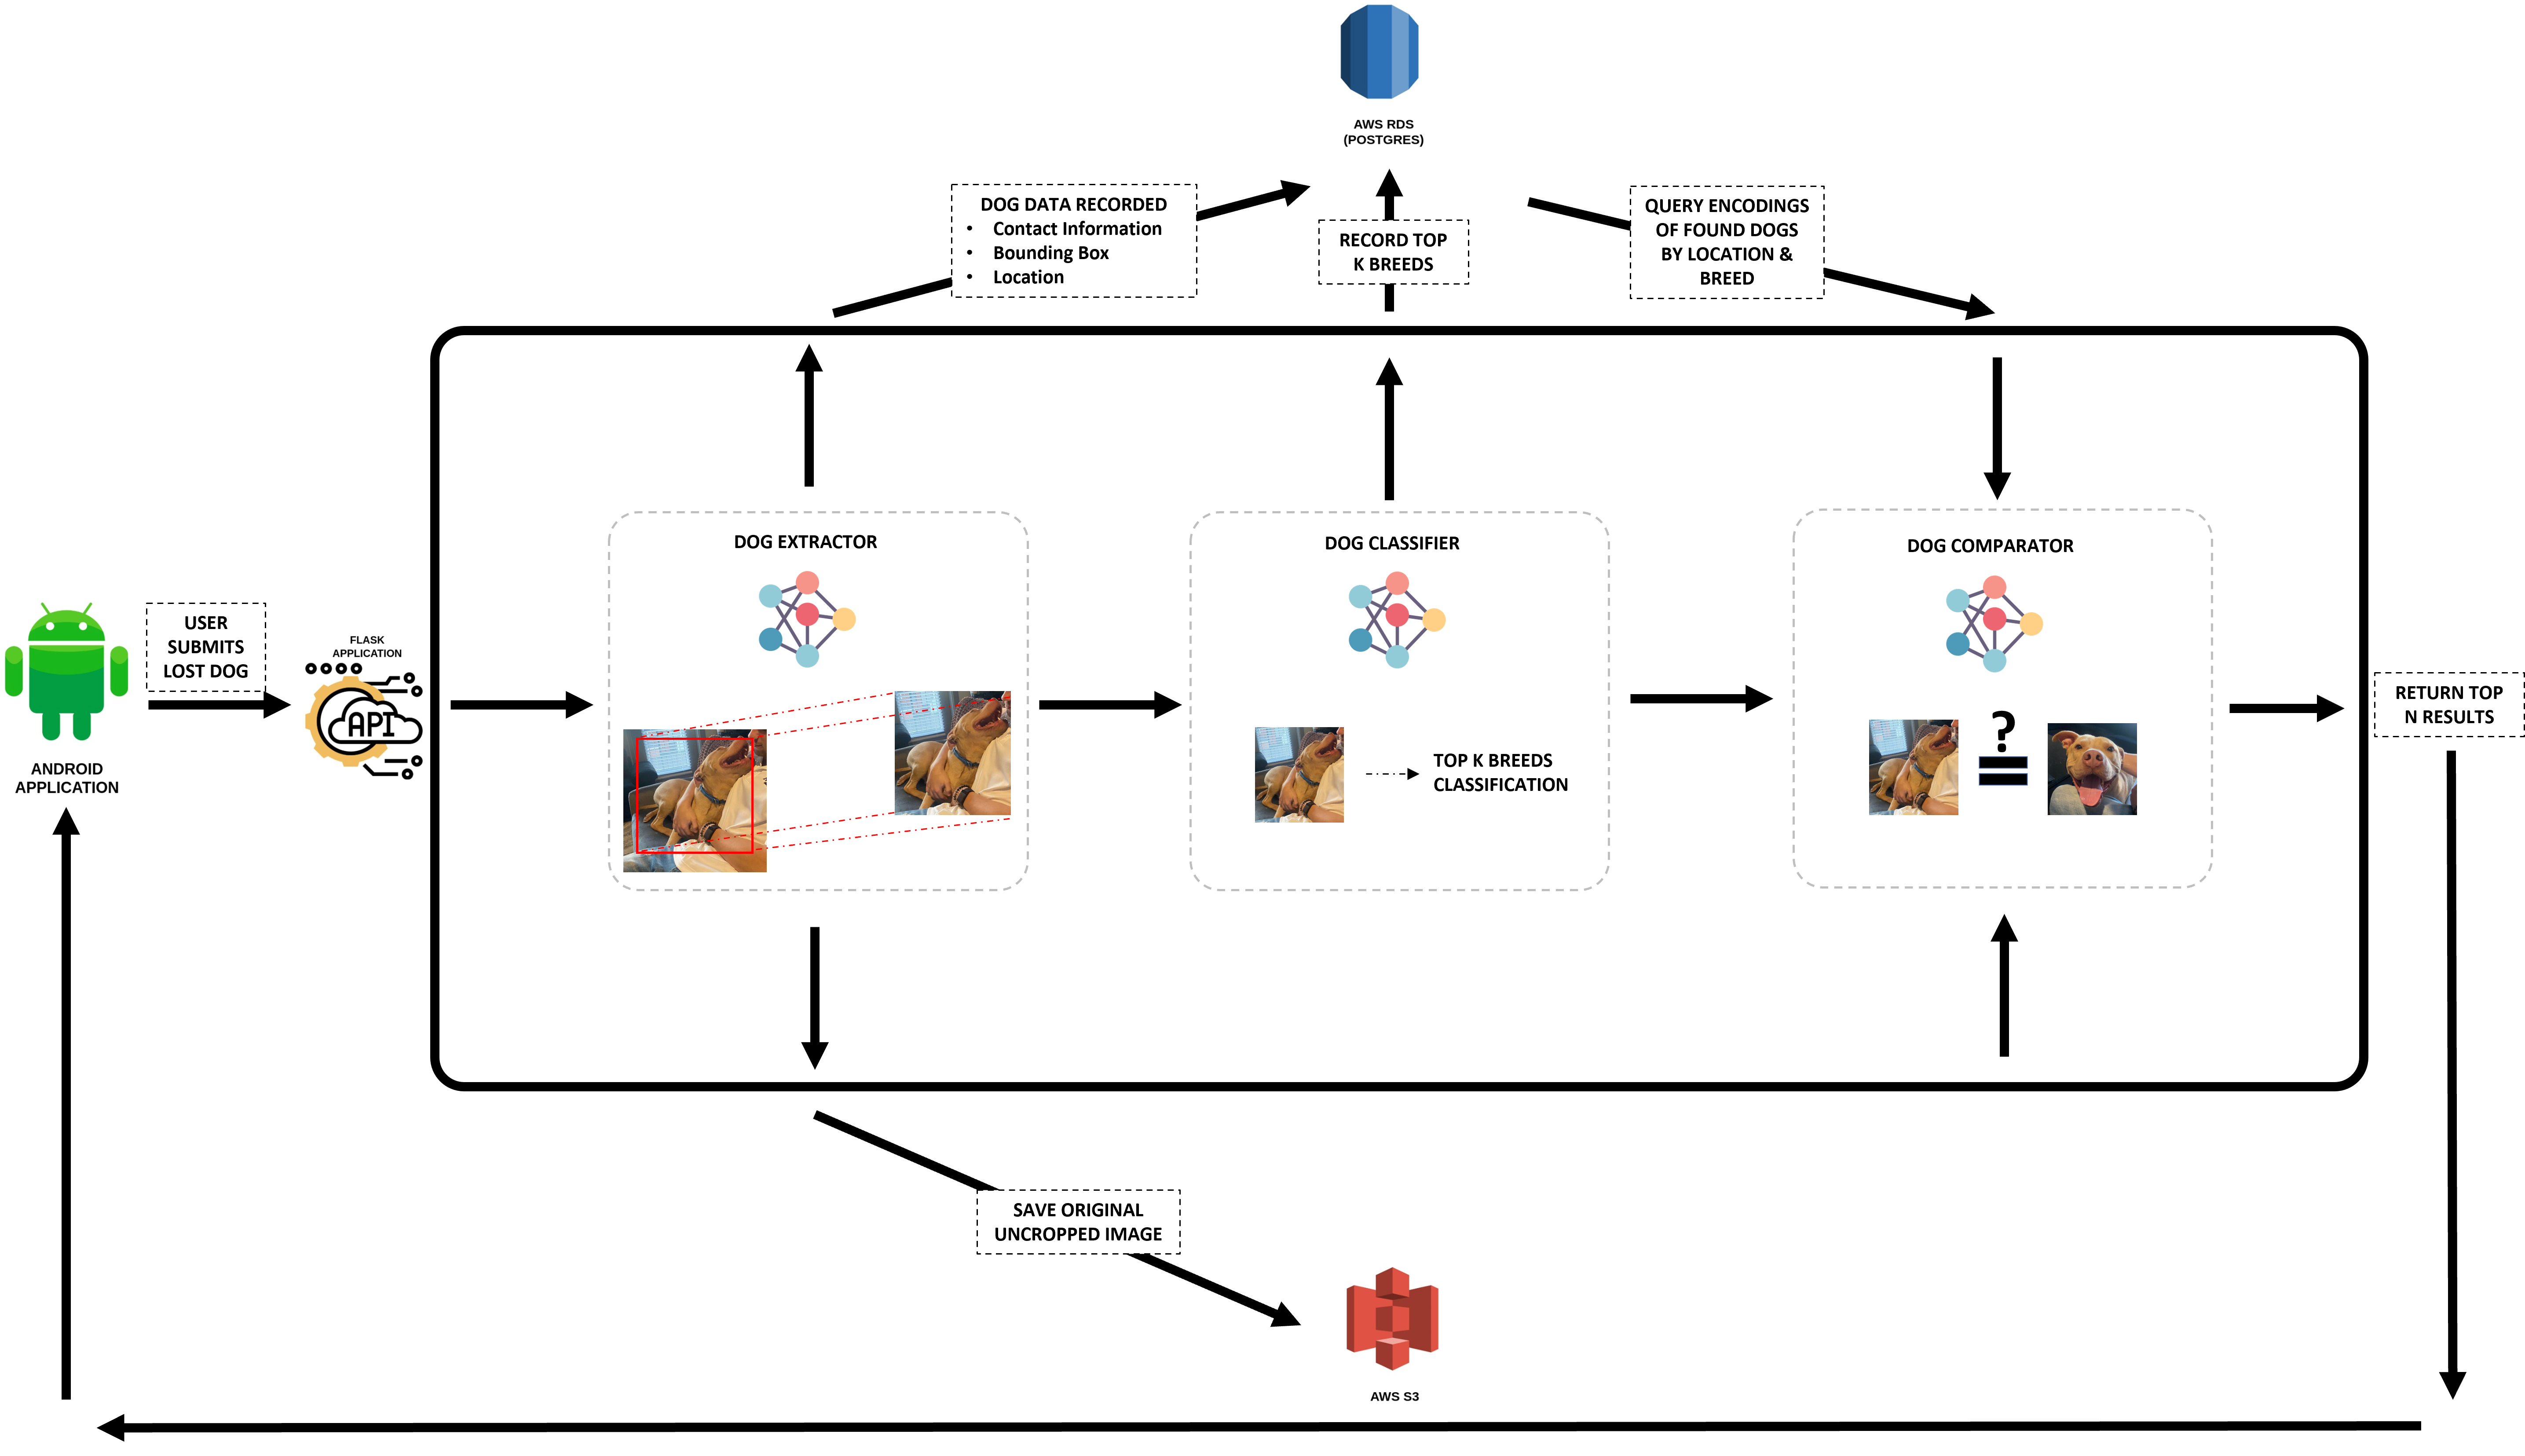
\includegraphics[width=1.0\textwidth]{final-report-images/applowlevel.png}
\caption{Dog Finder Pipeline}
\label{fig:x app pipeline}
\end{figure}

\begin{enumerate}
  
  \item Once a lost dog has been submitted, the image is passed to the "Dog Extractor" model that computes the coordinates of the bounding box of the dog.  This model also acts as a quality control by validating the image to ensure that the image contains a dog, and contains only one dog.  If these conditions are not met, an error is returned to the user.
  
  \item After validation, the original image is saved into an S3 bucket, and the related information such as the users contact information, location and the coordinates of the bounding box is inserted into a RDS.
  
  \item The original image is then cropped using the computed bounding box coordinates, and passed into the "Dog Classifier" model that computes the top $k$ most likely breeds.  This information is inserted into the RDS.
  
  \item We then query the dogs marked as found according to breed and location, and compare against the lost dog by passing the cropped image of each dog respectively into the "Dog Comparator" model.  The top $n$ results are returned to the user.
  
  \item If a match is confirmed by the user, the corresponding lost and found dogs are removed from the RDS and S3 bucket.  Otherwise, the lost dog is left in the system for future comparisons.
  
\end{enumerate}

An attentive reader will notice that we discuss only the submission of lost dogs.  This is done to minimize confusion.  If the user submits a found dog the pipeline is identical except that the dog is instead marked as found and is compared against dogs marked as lost.  This completes the pipeline contained within the application.  However, each model will be discussed in detail individually in the sections below.


\subsection{Dog Comparator}













\end{document}
